\section{Chapter 4: Labor Market Equilibrium}

This chapter will study the notion of labor market equilibrium,
which is the outcome of the interaction between labor supply, labor demand,
and possibly external forces, such as government policies.


\begin{definition}[Invisible Hand Theorem] 
    
    If markets are competitive, and workers and 
    firms are free to enter and leave the market, then 
    the equilibrium allocation of workers and wages 
    will be efficient, in the sense that it maximizes 
    the total gains that workers and firms 
    obtain from trade with each other.

\end{definition}

%%%%%%%%%%%%%%%%%%%%%%%%%%%%%%%%%%%%%%%%%%%%%%%%%%%%%%%%%%%%%%%%%%%%%%%%%%%%%%%%%%%%%%%
%%%%%%%%%%%%%%%%%%%%%%%%%%%%%%%%%%%%%%%%%%%%%%%%%%%%%%%%%%%%%%%%%%%%%%%%%%%%%%%%%%%%%%%
\subsection{Equilibrium in a Single Labor Market}

\autoref{fig:ch_4p1_surplus}
illustrates a competitive labor market with an 
equilibrium at $(E^*, w^*)$.


\FloatBarrier

\begin{figure}[!htb]
    \centering
        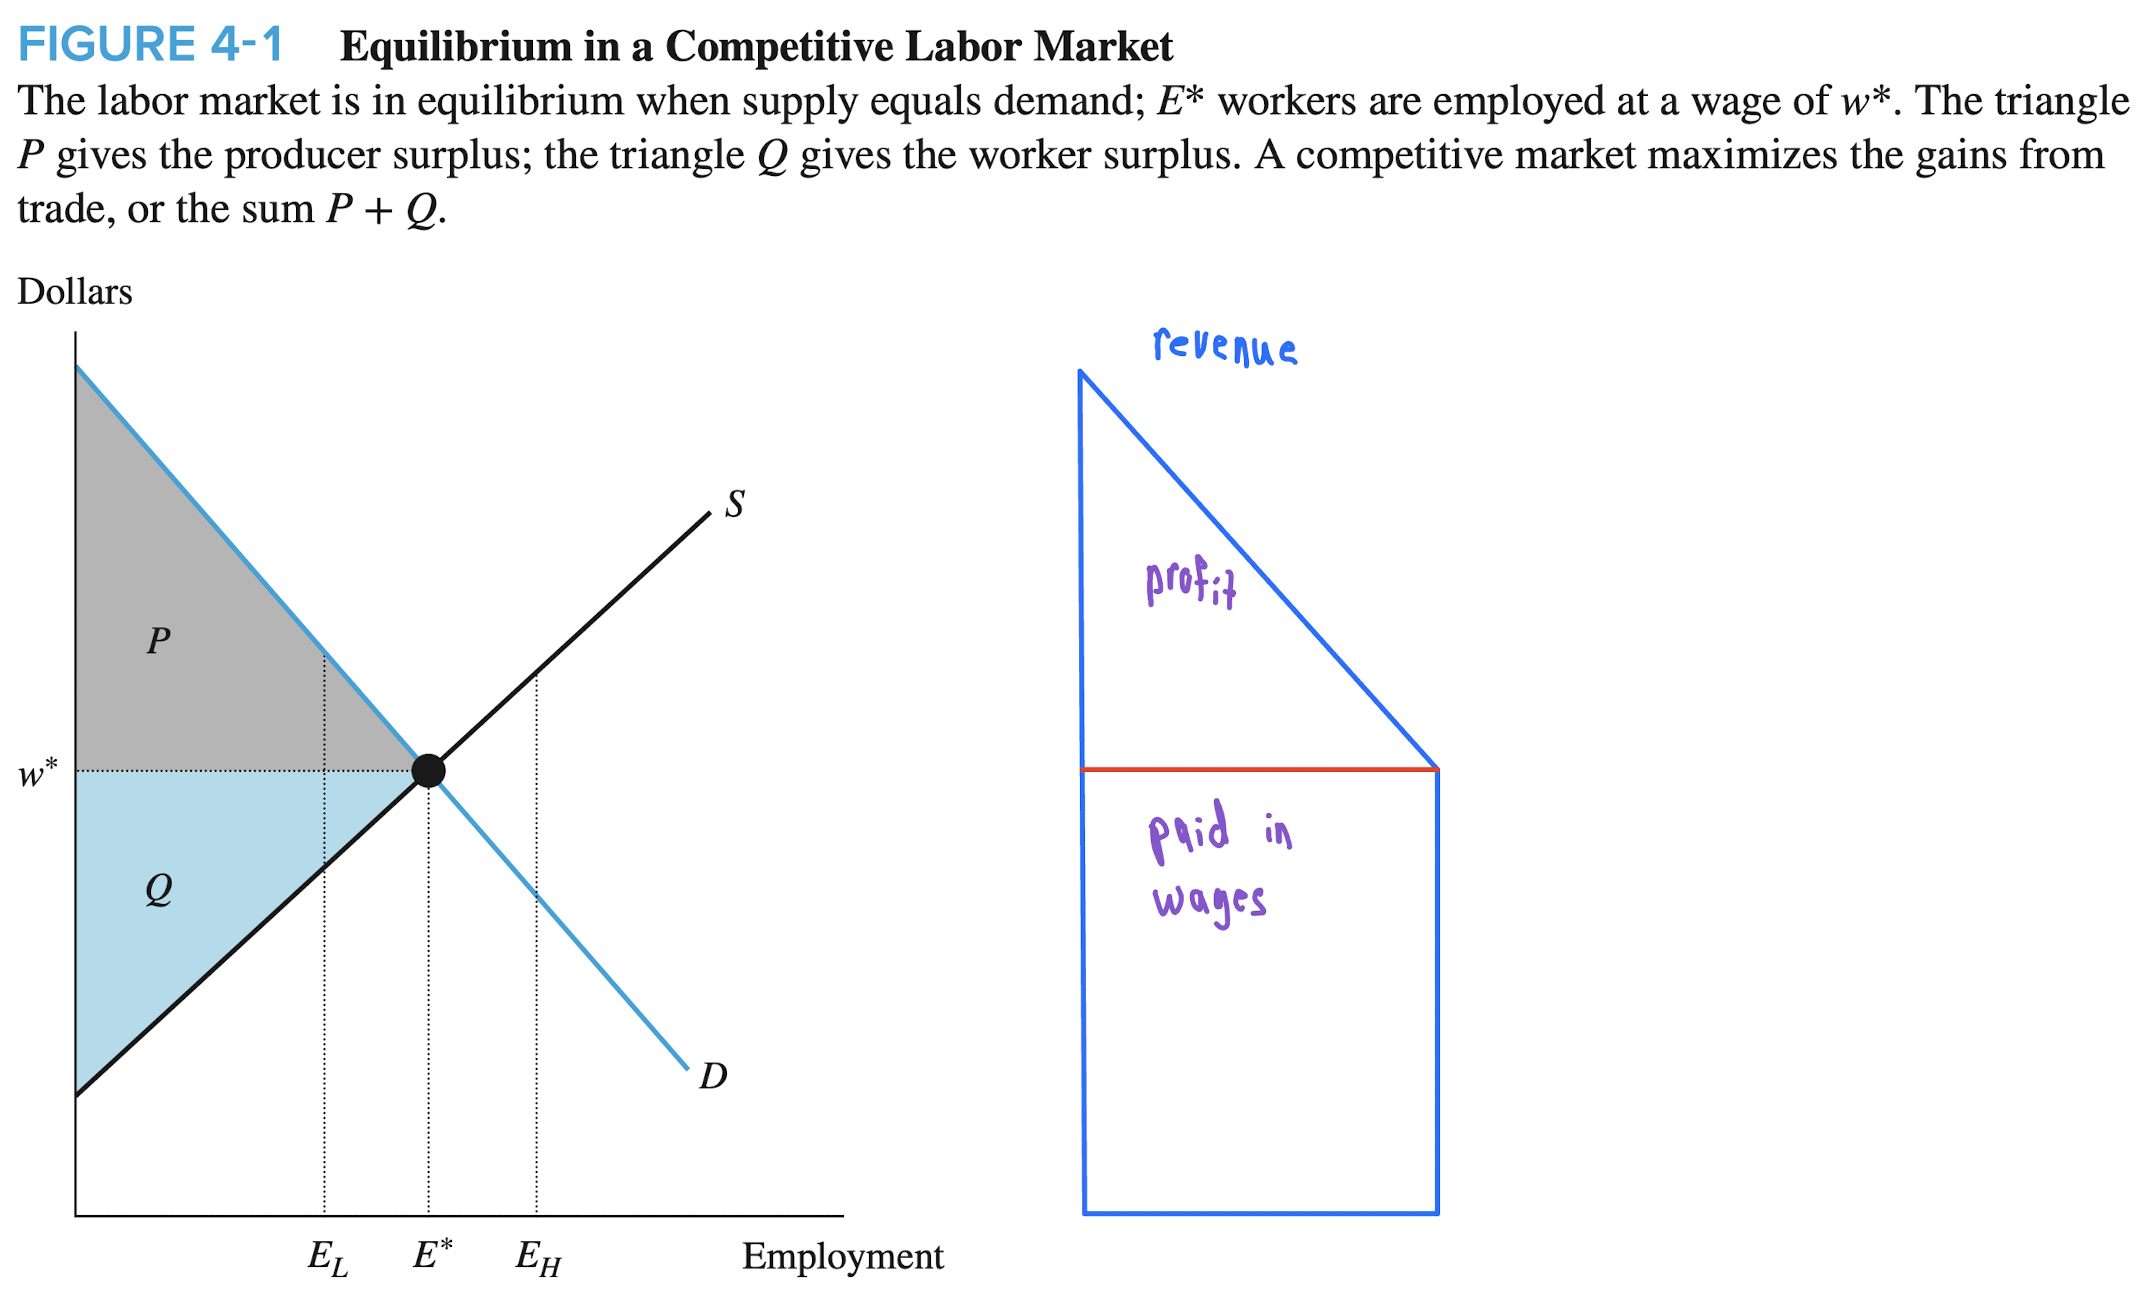
\includegraphics[width=0.95\textwidth]{../input/ch_4p1_surplus.png}
    \caption{Labor Market Surplus}
    \label{fig:ch_4p1_surplus}
\end{figure}

\FloatBarrier

Since the labor demand curve corresponds to the value of 
the marginal product, we can see that the area under the labor 
demand curve up to any given point corresponds to the total revenue
a firm receives from hiring that many workers.
Thus, since the equilibrium is at $(E^*, w^*)$, the
firm's total revenue is given by the area under the demand 
curve up to $E^*$, which is drawn out 
in blue in \autoref{fig:ch_4p1_surplus}.
Similarly, the area under the supply curve up to $E^*$,
their profit, or producer surplus (denoted $P$ in \autoref{fig:ch_4p1_surplus}), is 
given by the triangle above $w^*$ and below the labor 
demand curve.

\begin{definition}[Producer Surplus] 

    Producer surplus is the difference between the 
    revenue a firm receives and the cost it incurs.
    
\end{definition}

Similarly, workers are indifferent between working and not working 
along the labor supply curve. Thus, workers who are 
willing to work for less than $w^*$ (which is everyone 
except the final workers hired) receive a surplus.
This surplus is given by the triangle below $w^*$ and
above the labor supply curve, denoted $Q$ in 
\autoref{fig:ch_4p1_surplus}.

The gains from trade are given by the sum of the
producer and worker surplus: $P + Q$.
The competitive market equilibrium maximizes the 
gains from trade. Such an outcome that maximizes 
gains from trade is said to be ``efficient.''

\begin{questions}
    It's somewhat challenging for me to think about 
    how I should think about the connection between surplus 
    and wellbeing. I understood surplus as a clear quantitative 
    measure, but it seems like we would only care about it insofar as it 
    connects to something more like the wellbeing of the parties 
    involved. However, it's super unclear to me 
    if we're trying to connect it back to that 
    in any way.
\end{questions}

%%%%%%%%%%%%%%%%%%%%%%%%%%%%%%%%%%%%%%%%%%%%%%%%%%%%%%%%%%%%%%%%%%%%%%%%%%%%%%%%%%%%%%%
%%%%%%%%%%%%%%%%%%%%%%%%%%%%%%%%%%%%%%%%%%%%%%%%%%%%%%%%%%%%%%%%%%%%%%%%%%%%%%%%%%%%%%%
\subsection{Equilibrium across Labor Markets}

So far, we have focused on a single labor market.
Now, we turn to the case of multiple labor markets
linked by migration.
In \autoref{fig:ch_4p2_multiple_markets},
we see two labor markets, $N$ (north) and $S$ (south).
We start with the wages ($w_n$) in the north being 
higher than the wages ($w_s$) in the south.
If workers are able to move freely, then workers 
from the South will move to the North, which will
decrease supply in the South and increase supply
in the North up to the point that wages are equalized
across the two markets, at $w^*$.
Note that this analysis relies on the idea that workers 
in each region are perfect substitutes for each other.

We find that this movement 
increases the total output across the markets.
Specifically, the North market's 
output is originally the area under the demand curve 
up to $A$ and after the move extends to $B$ -- the 
increase is characterized by the blue trapezoid.
For the South, output reduces by the amount characterized 
by the blue trapezoid in its market. However,
the increase in the North is larger than the decrease
in the South. In particular, the growth in the North
is large by the size of the triangle $ABC$.


\FloatBarrier

\begin{figure}[!htb]
    \centering
        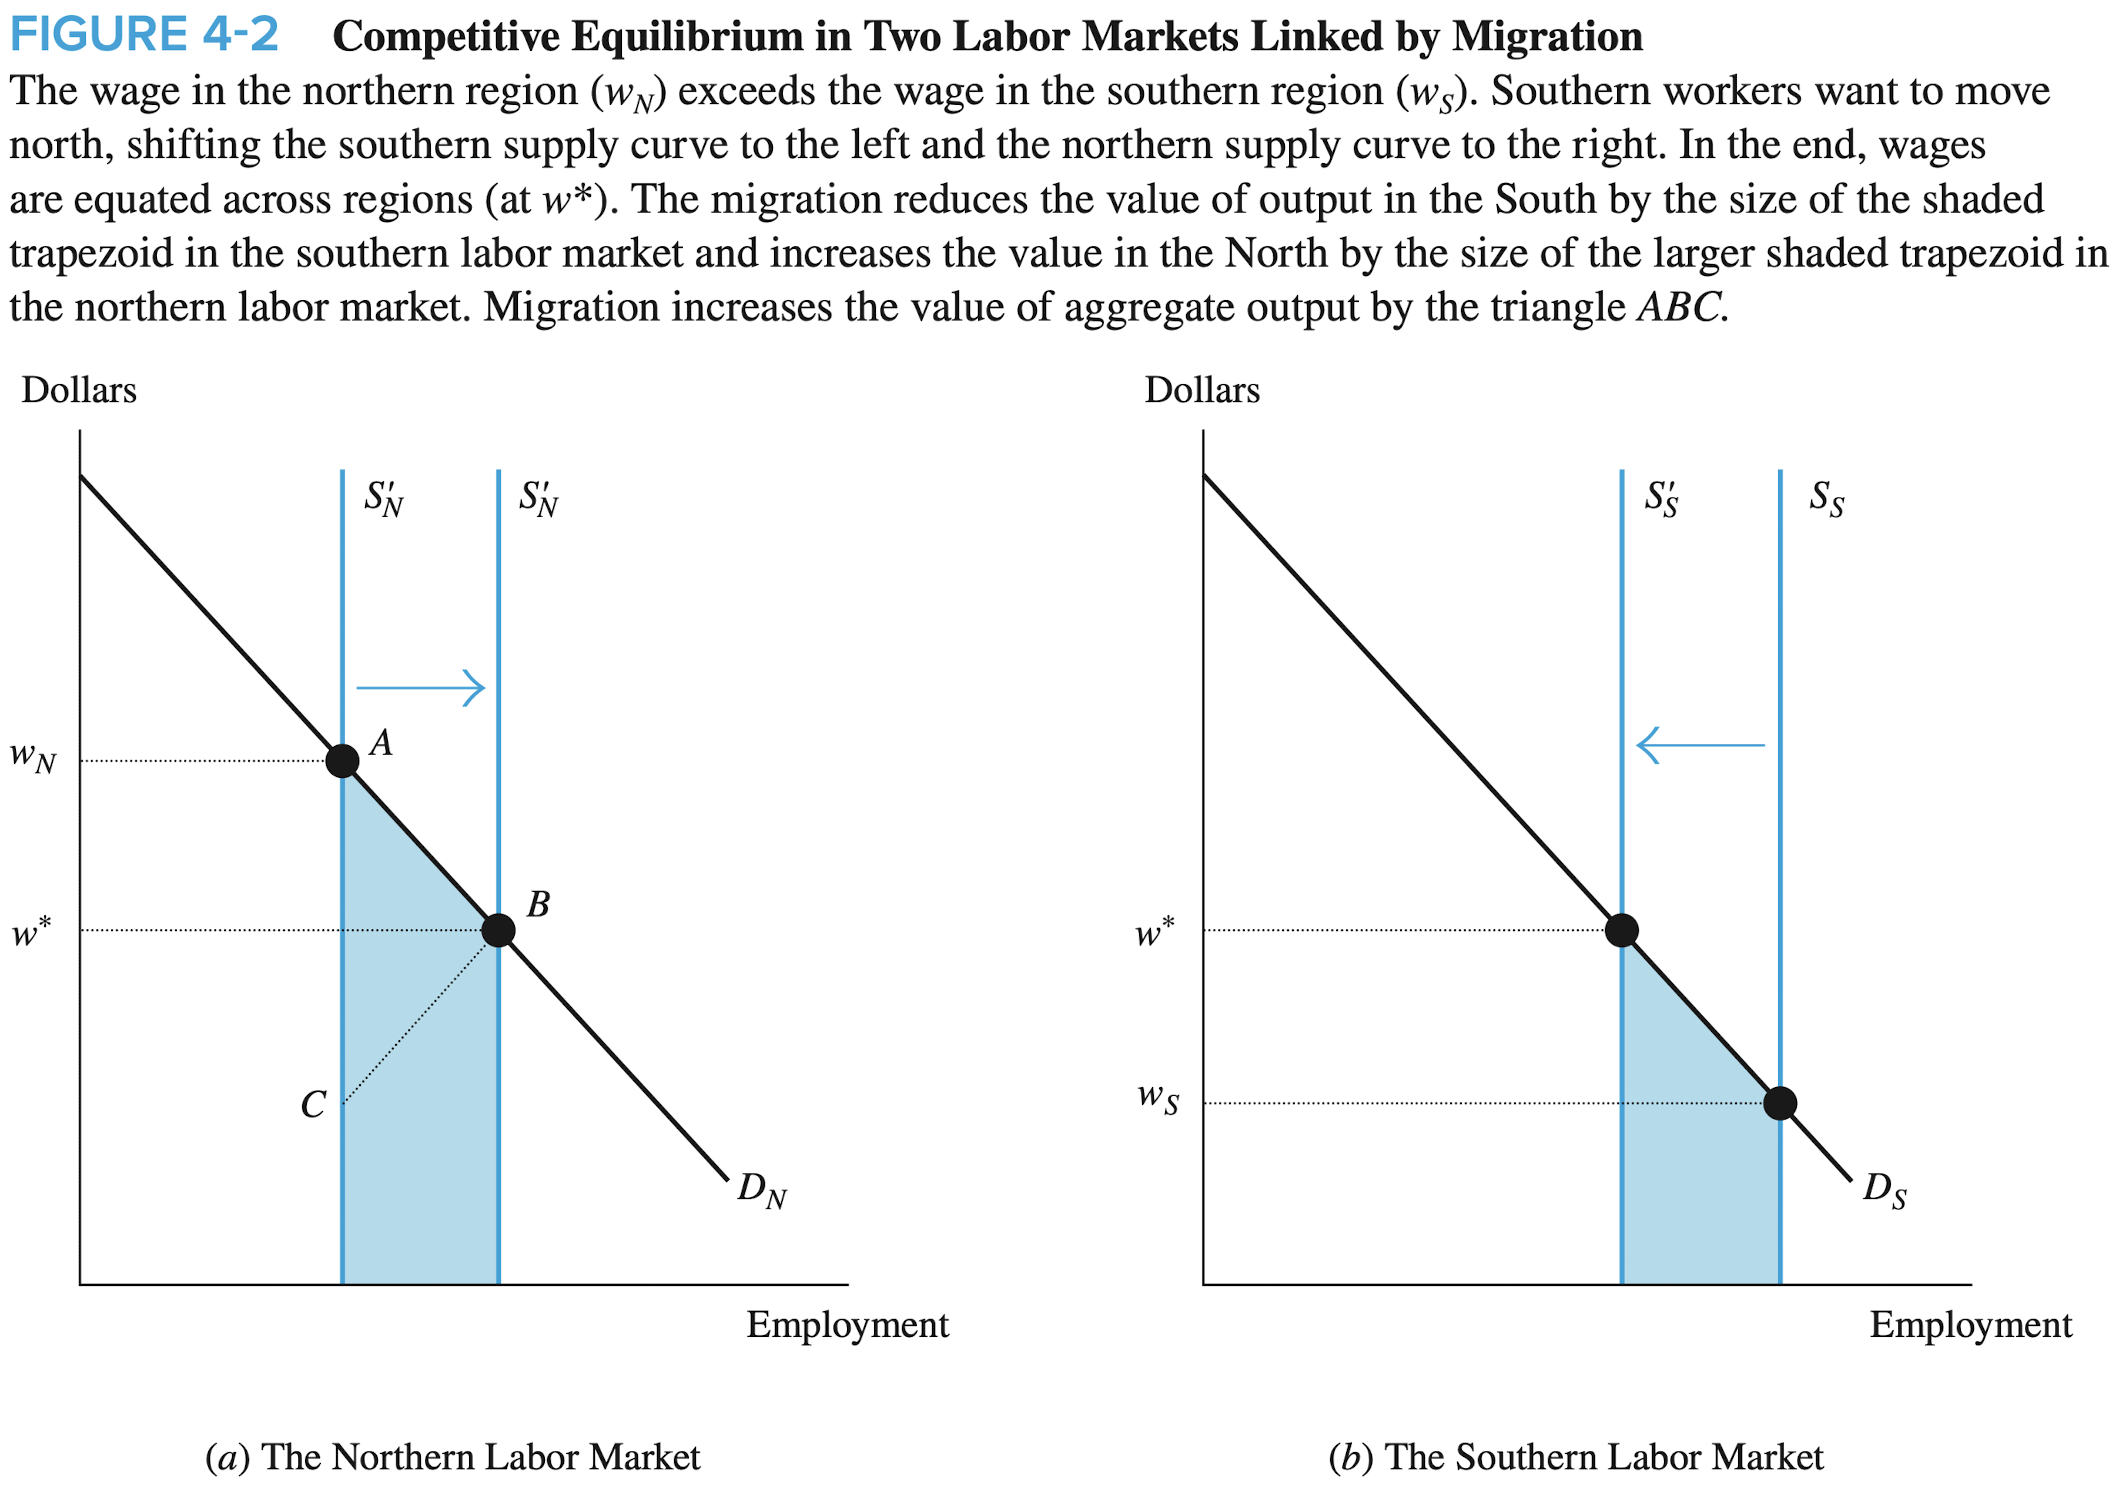
\includegraphics[width=0.95\textwidth]{../input/ch_4p2_multiple_markets.png}
    \caption{Equilibrium across Labor Markets}
    \label{fig:ch_4p2_multiple_markets}
\end{figure}

\FloatBarrier


%%%%%%%%%%%%%%%%%%%%%%%%%%%%%%%%%%%%%%%%%%%%%%%%%%%%%%%%%%%%%%%%%%%%%%%%%%%%%%%%%%%%%%%
%%%%%%%%%%%%%%%%%%%%%%%%%%%%%%%%%%%%%%%%%%%%%%%%%%%%%%%%%%%%%%%%%%%%%%%%%%%%%%%%%%%%%%%
\subsection{Policy Application: Payroll Taxes and Subsidies}

\subsubsection{Payroll Taxes Imposed on the Firm}

The payroll tax is a tax imposed on the firm 
that is some fraction $\tau$ of the wage paid to
the worker.

\autoref{fig:ch_4p3_payroll_tax}
illustrates the effect of a payroll tax.
Here, we suppose there is a payroll tax of \$1 per hour.
The initial equilibrium is at $(E_0, w_0)$, at point $A$.
The payroll tax placed on the firm decreases
the labor demand uniformly by the amount of the tax.
Thus, the new equilibrium is at point $B$, where 
the employment level is now $E_1$, the wage received 
by the worker is $w_1$, and the effective wage paid by 
the firm is $w_1 + 1$.

\FloatBarrier

\begin{figure}[!htb]
    \centering
        \includegraphics[width=0.95\textwidth]{../input/ch_4p3_payroll_tax.png}
    \caption{Payroll Tax}
    \label{fig:ch_4p3_payroll_tax}
\end{figure}

\FloatBarrier

%%%%%%%%%%%%%%%%%%%%%%%%%%%%%%%%%%%%%%%%%%%%%%%%%%%%%%%%%%%%%%%%%%%%%%%%%%%%%%%%%%%%%%%
\subsubsection{Payroll Taxes Imposed on the Worker}

\autoref{fig:ch_4p3_payroll_tax_worker}
illustrates the effect of a payroll tax
if it were imposed on the worker instead of the firm.
Here, the effect is essentially the reverse
in which the labor supply curve shifts up 
by the amount of the tax.
Now, the equilibrium is 
at point $B$, where the employment level is $E_1$,
the wage received by the worker is $w_1$, but 
the worker now pays a tax such that the 
effective wage received by the worker becomes $w_1 - 1$.

Whether the tax is imposed on the firm or the worker,
the outcome is the same.

\FloatBarrier

\begin{figure}[!htb]
    \centering
        \includegraphics[width=0.95\textwidth]{../input/ch_4p3_payroll_tax_worker.png}
    \caption{Payroll Tax Imposed on Workers}
    \label{fig:ch_4p3_payroll_tax_worker}
\end{figure}

\FloatBarrier

%%%%%%%%%%%%%%%%%%%%%%%%%%%%%%%%%%%%%%%%%%%%%%%%%%%%%%%%%%%%%%%%%%%%%%%%%%%%%%%%%%%%%%%

\subsubsection{When Will the Payroll Tax Be Shifted Completely to Workers?}

When the labor supply is perfectly inelastic,
the entire burden of the payroll tax is shifted to the worker,
as illustrated in \autoref{fig:ch_4p3_inelastic_and_payroll}.

\FloatBarrier

\begin{figure}[!htb]
    \centering
        \includegraphics[width=0.95\textwidth]{../input/ch_4p3_inelastic_and_payroll.png}
    \caption{When Payroll Tax is Shifted Completely to Workers}
    \label{fig:ch_4p3_inelastic_and_payroll}
\end{figure}

\FloatBarrier

%%%%%%%%%%%%%%%%%%%%%%%%%%%%%%%%%%%%%%%%%%%%%%%%%%%%%%%%%%%%%%%%%%%%%%%%%%%%%%%%%%%%%%%

\subsubsection{Deadweight Loss}

\autoref{fig:ch_4p3_deadweight_loss}
displays the reduction in the total surplus -- aka the deadweight loss --
that results from the imposition of a payroll tax.
Recall that the initial equilibrium is at $(E_0, w_0)$,
and the new equilibrium after the tax is at $(E_1, w_{\text{NET}})$,
where the firm pays $w_{\text{TOTAL}}$ and the worker receives $w_{\text{NET}}$.
Now, the total surplus has been reduced by the $DL$ triangle.
The consumer surplus now becomes
$Q^*$, rather than $Q$; the producer surplus now 
becomes $P^*$, rather than $P$; and the government
collects tax revenue equal to the rectangle $T$.

If you look back at \autoref{fig:ch_4p3_inelastic_and_payroll},
you can see that when the labor supply is perfectly inelastic,
there is no deadweight loss from the imposition of the tax,
and the producer surplus remains the same. 
All that changes is a transfer of consumer surplus to 
the government in the form of tax revenue. Specifically,
the rectangle characterized by $w_0AB(w_0 - 1)$
is transferred from consumer surplus to government revenue.


\FloatBarrier

\begin{figure}[!htb]
    \centering
        \includegraphics[width=0.95\textwidth]{../input/ch_4p3_deadweight_loss.png}
    \caption{Deadweight Loss}
    \label{fig:ch_4p3_deadweight_loss}
\end{figure}

\FloatBarrier


%%%%%%%%%%%%%%%%%%%%%%%%%%%%%%%%%%%%%%%%%%%%%%%%%%%%%%%%%%%%%%%%%%%%%%%%%%%%%%%%%%%%%%%
\subsubsection{Employment Subsidies}

\autoref{fig:ch_4p3_employment_subsidy}
illustrates the effect of an employment subsidy of \$1.
Effectively, this does the opposite of 
the payroll tax in terms of its effect on the 
demand curve; that is, the demand curve uniformly moves up 
by the size of the subsidy.

Under this setup, the equilibrium moves from $A$ to $B$, where 
at $B$, the worker receives a wage of $w_1$, while the firm 
only has to pay $w_1 -1$.


\FloatBarrier

\begin{figure}[!htb]
    \centering
        \includegraphics[width=0.95\textwidth]{../input/ch_4p3_employment_subsidy.png}
    \caption{Employment Subsidy}
    \label{fig:ch_4p3_employment_subsidy}
\end{figure}

\FloatBarrier

The effect of the subsidy on employment will 
depend both on the labor supply elasticity 
and the labor demand elasticity.
How it depends on the labor supply elasticity may 
be intuitive; if workers are 
very responsive to an increase in the wage, then 
more employment will be generated by the subsidy, and 
vice versa.

\autoref{fig:ch_4p3_demand_elas_impact} is a very quick 
demonstration that I draw of how the 
demand elasticity also impacts the effect on employment.
For example, in the first panel, if demand is perfectly inelastic, then 
the subsidy naturally has no effect on employment.
In the second panel, if demand is 
reasonably elastic, then the subsidy may have a more 
notable impact. The third panel shows the 
smaller effect when demand is reasonably inelastic 
but not perfectly inelastic.

\FloatBarrier
\begin{figure}[!htb]
    \centering
        \includegraphics[width=0.5\textwidth]{../input/ch_4p3_demand_elas_impact.png}
    \caption{Impact of Demand Elasticity on Employment}
    \label{fig:ch_4p3_demand_elas_impact}
\end{figure}
\FloatBarrier

%%%%%%%%%%%%%%%%%%%%%%%%%%%%%%%%%%%%%%%%%%%%%%%%%%%%%%%%%%%%%%%%%%%%%%%%%%%%%%%%%%%%%%%
%%%%%%%%%%%%%%%%%%%%%%%%%%%%%%%%%%%%%%%%%%%%%%%%%%%%%%%%%%%%%%%%%%%%%%%%%%%%%%%%%%%%%%%
\subsection{Policy Application: Mandated Benefits}

The government can assure every worker gets a 
certain benefit by mandating it.
How does this affect equilibrium 
wages and employment?

The book uses the example of mandating a 
spinach pie for every worker at lunch.

\autoref{fig:ch_4p4_mand_ben_effect}
depicts the effect of the mandatory benefit.
Suppose the mandated benefit costs $C$
dollars for the firm to provide, and the workers value it 
at $B$ dollars.
The demand curve shifts 
down uniformly by $C$, since they have to pay an extra $C$ dollars 
per worker. At the same time, the supply curve 
shifts down uniformly by $B$, since they will get an extra 
$B$ dollars of value.
In the first case, where $C > B$, 
displayed in Panel (a), the shift in supply doesn't offset 
the shift in demand, so employment is lower than before
the mandate, but not by as much as if a payroll tax had been implemented,
since the payroll tax would've involved only the downward shift in demand,
with no offsetting shift in supply.
If $C=B$, as in Panel (b), then the shifts cancel out,
and there is no effect on employment.


\FloatBarrier
\begin{figure}[!htb]
    \centering
        \includegraphics[width=0.95\textwidth]{../input/ch_4p4_mand_ben_effect.png}
    \caption{Effect of Mandated Benefits}
    \label{fig:ch_4p4_mand_ben_effect}
\end{figure}
\FloatBarrier

The textbook highlights that the mandated benefit 
reduces the deadweight loss relative to a payroll tax
when $B > 0$ and says that this means we prefer 
mandated benefits to payroll taxes.

\begin{questions}
    I am a bit confused by the last claim. It seems like 
    if $B >0 $ narrowly and $C$ is much larger than $B$,
    then we have this scenarios where we basically
    burn a lot of money and don't even get tax revenue for it.
    This seems like the distortion triangle is smaller, which
    seems to be the author's point, but the fact that we've traded 
    a lot of tax revenue for burned money seems like 
    it would make the overall welfare effect negative.
    Am I thinking about this wrong?
\end{questions}

%%%%%%%%%%%%%%%%%%%%%%%%%%%%%%%%%%%%%%%%%%%%%%%%%%%%%%%%%%%%%%%%%%%%%%%%%%%%%%%%%%%%%%%
%%%%%%%%%%%%%%%%%%%%%%%%%%%%%%%%%%%%%%%%%%%%%%%%%%%%%%%%%%%%%%%%%%%%%%%%%%%%%%%%%%%%%%%
\subsection{The Labor Market Impact of Immigration}

\subsubsection{The Simplest Version}

In the simplest model of analyzing the 
impact of immigration, we suppose that 
native and immigrant workers are perfect substitutes.

Panel (a) \autoref{fig:ch_4p5_imm_eff_simple} 
illustrates the impact of immigration 
under this assumption. Essentially,
immigration constitutes a positive 
supply shock, which increases employment 
and reduces wages.

In contrast, if native and immigrant labor 
are complements, e.g., if the presence of 
immigrant workers permits native workers 
to specialize in tasks in which they are more adept,
then this would correspond to a positive demand shock for native workers, 
as demonstrated in Panel (b) of \autoref{fig:ch_4p5_imm_eff_simple}.
In this case, both employment and wages
of native workers increase.


\FloatBarrier

\begin{figure}[!htb]
    \centering
        \includegraphics[width=0.95\textwidth]{../input/ch_4p5_imm_eff_simple.png}
    \caption{Impact of Immigration on Labor Market - Simplest Version}
    \label{fig:ch_4p5_imm_eff_simple}
\end{figure}

\FloatBarrier

%%%%%%%%%%%%%%%%%%%%%%%%%%%%%%%%%%%%%%%%%%%%%%%%%%%%%%%%%%%%%%%%%%%%%%%%%%%%%%%%%%%%%%%
\subsubsection{The Short Run and the Long Run}

Suppose again that native and immigrant workers 
are perfect substitutes. What happens in the short run? 
As considered above, the supply curve shifts out,
employment increases, and wages decrease.
This decrease in worker wages and increase in workers
will raise the returns to capital and increase profits. 
Thus, in the long run, firms will invest more in capital,
as existing firms expand and new firms enter the market 
to take advantage of the cheap labor.
The increase in the capital stock 
will then 
shift the labor demand curve to the right, attenuating the 
effects of the initial supply shock.
However, by how much will the demand curve shift to the right 
in the long run?
The answer depends on the production technology.

As an example, suppose we have a Cobb-Douglas production function:

\begin{align}
    q=A K^\alpha E^{1-\alpha}
\end{align}

where

\begin{itemize}
    \item $A$: total factor productivity
    \item $K$: capital
    \item $E$: labor
    \item $\alpha \in (0,1)$
\end{itemize}

This production function has constant returns to scale;
that is, if we double both $K$ and $E$, then output $q$ will also double.

Recall that the profit-maximizing conditions in 
a competitive market require that 
the price of capital ($r$) and the price of labor ($w$)
are equal to their respective value of their marginal products.
Thus, the marginal productivity conditions for 
the Cobb-Douglas production function are: 

\begin{align}
    &r=M P_k p \quad \& \quad M P_k=\alpha A K^{\alpha-1} E^{1-\alpha}
    \Rightarrow &&r=\$ 1 \times \alpha A K^{\alpha-1} E^{1-\alpha} \\
    &w=M P_e p \quad \& \quad M P_e=(1-\alpha) A K^{\alpha} E^{-\alpha}
    \Rightarrow &&w=\$ 1 \times (1-\alpha) A K^{\alpha} E^{-\alpha}
\end{align}

We can re-write this as:

\begin{align}
    r & =\alpha A\left(\frac{K}{E}\right)^{\alpha-1}=\alpha A\left(\frac{E}{K}\right)^{1-\alpha} \label{eq:ch4_rental_cobb_douglas} \\
    w & =(1-\alpha) A\left(\frac{K}{E}\right)^\alpha
\end{align}

The marginal product of capital is increasing with the number of 
workers (and hence so is the value of the marginal product of capital).
Thus, as the number of workers increases, the demand for capital increases.
Similarly, the marginal product of labor is increasing with the amount of
capital (and hence so is the value of the marginal product of labor).
Thus, as the amount of capital increases, the demand for labor increases.

If we suppose the $r$ is fixed, then \eqref{eq:ch4_rental_cobb_douglas}
implies that the ratio of $E/K$ is fixed.
Thus, in this case, it must be that in the long run, 
the wage returns to its initial level.
See \autoref{fig:ch_4p5_long_run_imm}
for an illustration of this case.

\FloatBarrier

\begin{figure}[!htb]
    \centering
        \includegraphics[width=0.95\textwidth]{../input/ch_4p5_long_run_imm.png}
    \caption{Long Run Effects of Immigration on Labor Market}
    \label{fig:ch_4p5_long_run_imm}
\end{figure}

\FloatBarrier

%%%%%%%%%%%%%%%%%%%%%%%%%%%%%%%%%%%%%%%%%%%%%%%%%%%%%%%%%%%%%%%%%%%%%%%%%%%%%%%%%%%%%%%
\subsubsection{The Immigration and Minimum Wage Debates}

One interesting point is that the 
immigration and minimum wage debates are both 
focused on the labor demand elasticity.
When we consider the results together, we should 
consider what certain pairs of results imply. 
For example, if we take the results (discussed in the 
textbook, but not in my notes) that 
immigration had no effect on employment in the 
Mariel natural experiment and that 
the minimum wage had no effect on employment in the 
NJ-Pennsylvania natural experiment, 
then this implies that the short-run labor demand elasticity is
both perfectly elastic and perfectly inelastic,
as shown in \autoref{fig:ch_4p5_imm_min_wage_labor_demand}.
The author highlights the point that, though one can argue that 
these are simply different labor markets with different contexts, 
it would be troubling for the usefulness of
the empirical evidence, since it would imply that 
the results in one setting tell you nothing about the 
dynamics in 
another setting.


\FloatBarrier

\begin{figure}[!htb]
    \centering
        \includegraphics[width=0.95\textwidth]{../input/ch_4p5_imm_min_wage_labor_demand.png}
    \caption{Labor Demand Elasticity in Immigration and Minimum Wage Debates}
    \label{fig:ch_4p5_imm_min_wage_labor_demand}
\end{figure}

\FloatBarrier

%%%%%%%%%%%%%%%%%%%%%%%%%%%%%%%%%%%%%%%%%%%%%%%%%%%%%%%%%%%%%%%%%%%%%%%%%%%%%%%%%%%%%%%
%%%%%%%%%%%%%%%%%%%%%%%%%%%%%%%%%%%%%%%%%%%%%%%%%%%%%%%%%%%%%%%%%%%%%%%%%%%%%%%%%%%%%%%
\subsection{The Immigration Surplus}

The author notes that although immigration 
may have negative effects on the wages of competing workers, 
it may generate gains for the aggregate economy.
These gains come from the fact that the 
market wage equals the productivity of the last worker 
hired. Thus, all immigrants added to the economy, except 
for the last one, add more to the economy than they are paid.
This is illustrated in \autoref{fig:ch_4p6_imm_surplus},
where we take supply to be perfectly inelastic for the 
sake of simplicity.
In this case, the immigration surplus is given by
the triangle BCF. In fact, we can break up the 
segments further. Prior to the immigration supply shock, 
B reflects the equilibrium point, and 
the area ABN0 reflects the total output.
After the immigration supply shock, 
the new equilibrium is at C, and 
the total output becomes ACM0.
$w_0BFw_1$ is switched from 
being accrued in wages to 
being accrued in profits for the firms,
$BCF$ is the new output generated that flows 
to firms, and $CFMN$ is the new output generated that 
flows to the immigrant workers.
Thus, immigration in this simple model corresponds to 
a loss in wages for workers, a greater increase in profits for firms (greater 
by the amount of the immigration surplus),
and the introduction of new wages to the immigrants themselves.
In general, the immigration surplus can be calculated 
as 

\begin{align}
    \text{Immigration surplus} =\frac{1}{2} \times\left(w_0-w_1\right) \times(M-N)
\end{align}


\FloatBarrier

\begin{figure}[!htb]
    \centering
        \includegraphics[width=0.95\textwidth]{../input/ch_4p6_imm_surplus.png}
    \caption{Immigration Surplus}
    \label{fig:ch_4p6_imm_surplus}
\end{figure}

\FloatBarrier

\begin{questions}
    
    The book notes that, in the long run under 
    constant returns to scale, 
    the immigration surplus is zero. (GDP goes up but all the gains
    go to the immigrants.) I'm not sure if 
    I totally understand this yet.

\end{questions}

%%%%%%%%%%%%%%%%%%%%%%%%%%%%%%%%%%%%%%%%%%%%%%%%%%%%%%%%%%%%%%%%%%%%%%%%%%%%%%%%%%%%%%%
%%%%%%%%%%%%%%%%%%%%%%%%%%%%%%%%%%%%%%%%%%%%%%%%%%%%%%%%%%%%%%%%%%%%%%%%%%%%%%%%%%%%%%%
\subsection{Policy Application: High-Skill Immigration}

A supplementary theory introduces the notion that 
some immigrants, especially high-skill immigrants, 
may generate ``human capital externalities.''
That is, immigrants may introduce 
new ideas, ways of thinking, etc. that make 
native workers more productive than they 
otherwise would've been.
In this case, immigrants not only shift the supply curve, 
but also the demand curve, by shifting the 
value of the marginal product of labor.

\autoref{fig:ch_4p7_imm_surplus_amid_prod_extern}
illustrates this case. In this scenario,
the increase to natives' income is 
given by the sum of the areas of BCD and 
ABEF. In this case, wages and employment can both rise.


\begin{figure}[!htb]
    \centering
        \includegraphics[width=0.95\textwidth]{../input/ch_4p7_imm_surplus_amid_prod_extern.png}
    \caption{Immigration Surplus Amid Productivity Externalities}
    \label{fig:ch_4p7_imm_surplus_amid_prod_extern}
\end{figure}

\begin{notes}
    Some diagnostic questions:
    \begin{itemize}
        \item Whose supply and demand curves are we looking at? When we look at 
            a supply-demand diagram, we may be focusing on 
            a particular group of workers, e.g.,
            native workers in a particular skill group.
            This is important, as the effect of e.g., immigration or 
            the minimum wage may be different for different groups of workers.
            For example, the impact of immigrants might increase the supply 
            curve for one group of workers by being 
            substitutes for them, but increase the demand curve
            for another group of workers by being complements for them.
    \end{itemize}
\end{notes}

%%%%%%%%%%%%%%%%%%%%%%%%%%%%%%%%%%%%%%%%%%%%%%%%%%%%%%%%%%%%%%%%%%%%%%%%%%%%%%%%%%%%%%%
%%%%%%%%%%%%%%%%%%%%%%%%%%%%%%%%%%%%%%%%%%%%%%%%%%%%%%%%%%%%%%%%%%%%%%%%%%%%%%%%%%%%%%%
\subsection{The Cobweb Model}

